%!TEX TS-program = pdflatex

%%%% Latex preamble and page formatting %%%%

\documentclass[12pt]{article}  % larger font to compensate for long lines with fullpage
\usepackage[utf8]{inputenc}
\usepackage[T1]{fontenc}
\usepackage[pdfborder={0 0 0}]{hyperref} % use hyperref without borders
\usepackage{ifpdf}
\usepackage{ifthen}
\usepackage{graphicx}
\usepackage{url}
\usepackage{color}
\usepackage{listings}
\usepackage[title,titletoc]{appendix}
% Read pictures from img/ and current directory
\graphicspath{{img/}{./}}

%%% GWD/GFD header follows %%%
% Feel free to make changes, as long as your document follows the guidelines of GFP.152

\usepackage[numbers]{natbib} % Use [1] for references, 
\bibliographystyle{plainnat} % References show full author name(s) and document URL

\usepackage[sf,compact]{titlesec} % Use sans-serif for section headers

\usepackage[titles]{tocloft} % Format table of contents
% (tocloft is used, since titletoc is incompatible with xetex.)
\renewcommand{\cftsecfont}{\sffamily}
\renewcommand{\cftsubsecfont}{\sffamily}
\renewcommand{\cftsubsubsecfont}{\sffamily}
\renewcommand{\cftsecpagefont}{\sffamily}
\renewcommand{\cftsubsecpagefont}{\sffamily}
\renewcommand{\cftsubsubsecpagefont}{\sffamily}
\renewcommand{\cftsecleader}{\cftdotfill{\cftsubsecdotsep}} % dots for sections the same as for sections
\setlength{\cftbeforesecskip}{0.5ex}

\usepackage{parskip} % Blank lines between paragraphs, no indentation.

% font style for headers and footers
\newcommand{\headerstyle}{\sffamily} % sans-serif

% Set page margins
\usepackage{fancyhdr}
\addtolength{\headheight}{15pt}
\renewcommand{\headrulewidth}{0pt}
% \setlength{\headrulewidth}{0pt}
\setlength{\headsep}{20pt}
\usepackage[headings]{fullpage}  % small margins

% Macro to make some editorial notes
\newenvironment{note}{\framebox{note:} \color[gray]{0.5}}{}

% Macro to check if (optional) values above are defined or not.
\newcommand{\ifnonempty}[2]{\ifthenelse{\isundefined{#1}}{}{\ifthenelse{\equal{#1}{}}{}{#2}}}

%%%% Document header and title page %%%%

\title{Network Service Interface Topology Service Distribution Mechanisms}
\author{Jeroen van der Ham}
\newcommand{\shortdoctitle}{NSI TS}  % Title used in page header
% \date{} and \author{} are currently ignored
\newcommand{\authorsshort}{Jeroen van der Ham, UvA}
\newcommand{\publicationdate}{March 2013}  % Date of first publication of the document
% \newcommand{\revisiondate}{August 2012}  % Optional: date of last revision of the document
\newcommand{\copyrightyears}{2008-2013}  % Years used in copyright notice
\newcommand{\docseries}{GWD-I}  % GWD-R, GWD-I or GWD-C (for working drafts)
% \newcommand{\docseries}{GFD.191}  % GFD.000 (for approved documents)

\ifpdf
\hypersetup{
    pdftitle = {Network Service Interface Topology Service Distribution Mechanisms},
    pdfauthor = {Jeroen van der Ham},
    pdfsubject = {Description of distribution mechanisms for the topology service},
    pdfkeywords = {nsi topology distribution}
}
\fi


% Define page header and footers
\pagestyle{fancyplain}
\fancyhf{}
\lhead{\fancyplain{}{\headerstyle\docseries}}
% use \revisiondate if defined, otherwise \publicationdate for right header:
\rhead{\fancyplain{}{\headerstyle\ifthenelse{\isundefined{\revisiondate }}{\publicationdate}{\ifthenelse{\equal{\revisiondate}{}}{\publicationdate}{\revisiondate}}}}
\lfoot{\headerstyle\ifnonempty{\groupurl}{\groupurl}}
\rfoot{\headerstyle\thepage}
\thispagestyle{plain}

\begin{document}

% Title page header
{\noindent
\begin{minipage}[t]{1.5in}
\headerstyle
\docseries \\
NSI-WG \\
\href{mailto:nsi-wg@ogf.org}{nsi-wg@ogf.org}
\end{minipage}
\hfill
\raggedleft
\begin{minipage}[t]{4.5in}
\raggedleft
\headerstyle
\authorsshort \\
\vspace{1em}
\publicationdate \\
\ifnonempty{\revisiondate}{Revised \revisiondate \\}
\end{minipage}
}

\vspace{1em}
\begin{center}
\makeatletter
\Large\bf\textsf \@title
\makeatother
\end{center}


\section*{Status of This Document}

Group Working Draft (GWD), Informational (I).
% TODO: before publication:
%Grid Final Draft (GFD), Informational (I).


% \section*{Document Change History}
% 
% TODO: use this for formal revisions of this document

\section*{Copyright Notice}

Copyright \copyright \ Open Grid Forum (\copyrightyears).  Some Rights Reserved.  
Distribution is unlimited.

\phantomsection\addcontentsline{toc}{section}{Abstract}
\section*{Abstract}

This document describes a normative schema which allows the
description of service plane objects required for the Network Service Interface Connection Service. Additionally it describes a set of distribution mechanisms for the network topology descriptions.

\phantomsection\addcontentsline{toc}{section}{Contents}
\tableofcontents

\newcommand{\qq}{\symbol{34}} % 34 is the decimal LaTeX code for "
\newcommand{\q}{\symbol{39}} % 39 is the decimal LaTeX code for '
\newcommand{\underscore}{\symbol{95}} % 39 is the decimal LaTeX code for _

\newcommand{\MUST}{\textsc{must}}
\newcommand{\MUSTNOT}{\textsc{must not}}
\newcommand{\REQUIRED}{\textsc{required}}
\newcommand{\SHALL}{\textsc{shall}}
\newcommand{\SHALLNOT}{\textsc{shall not}}
\newcommand{\SHOULD}{\textsc{should}}
\newcommand{\SHOULDNOT}{\textsc{should not}}
\newcommand{\RECOMMENDED}{\textsc{recommended}}
\newcommand{\MAY}{\textsc{may}}
\newcommand{\OPTIONAL}{\textsc{optional}}

\newpage

\section{Representation of Network Topologies}\label{sec:representation}

In order to use the NSI Connection Service, some form of topology representation 
is required. In this section we explain the topology representation requirements for the NSI Connection Service. A diagram that provides some generic insight into NSI Topology is provided in figure~\ref{fig:ndgf}.

\begin{figure}[htbp]
\begin{center}
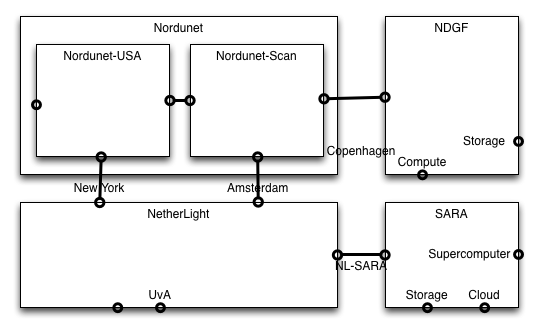
\includegraphics[width=390pt]{image00.png}
\caption{Abstract view of an example NSI Topology}\label{fig:ndgf}
\end{center}
\end{figure}


\subsection{Introduction to concept of STPs}

The basic network topology for the Network Service Interface (NSI) 
consists of networks, points and connections. The NSI can be used to request a 
connection between two different points, which is then implemented using the connection(s) 
between those points. Since each of the points in the network topology can terminate 
a network service, they are called Service Termination Points (STPs). The figure 
above contains several of these, for example the Storage point at SARA, another 
example is the connection point between the network on the edge of the SARA network 
which connects to the Netherlight network.


\subsection{Identifying STPs in a request}

The STPs in the Network Topology generally have two different 
roles:

\begin{itemize}
    \item  Endpoints within the network – points which are of interest to 
users, used as source and destination points

\item  One Part of a Service Demarcation Point (SDP) – meaning connections 
to other networks, used as transit points
\end{itemize}

For the NSI network service, knowledge of the connections between 
networks is necessary to enable pathfinding. It is not strictly necessary to know 
all of the user endpoints in a network, as long as it is known in which network 
the endpoint is. It is assumed that once the network is reached, the endpoint within 
the network can be reached as well.

To allow for pathfinding it is necessary that the Topology Service 
can identify the Networks, and the connections between those Networks, the SDPs. 
It is not necessary to distribute all of the endpoints within the network, which 
makes the distribution process much simpler.

This means that an NSI Connection Service reservation request must contain the source and destination 
network, as well as the connection points within those respective networks.


\subsection{Explicit routing using STPs}

In a regular request only the source and destination STPs and 
their networks are specified. The selected path between those STPs is left to the 
NSA managing the request. In NSI v2.0 it is also possible to steer the requested 
path into a specific direction by defining intermediate STPs that the path must 
touch.

Instead of a normal request with just a source and destination 
STP, the explicitly routed request will contain a path element which contains an 
indication of the path that should be taken through the NSI Network.

If the Path object contains a description of the complete path 
end-to-end then this is simply a question of availability. However, problems can 
arise if the path object only contains a single ``explicit route object''(ERO) 
that it must touch. With the current NSI implementation (v1) and its bi-directional 
model, there is no way to know from which way to cross that ERO. The proposal is 
to use uni-directional path elements, to avoid ambiguity in the path direction 
(the uni-directionality of the ERO implicitly defines the direction).


\subsection{Requirements for Topology Descriptions}

Taking the description above into account, and with the general 
idea of the Network Service Interface in mind, we come to the following requirements 
for the network topology description:

\begin{description}
    \item  \textbf{Scalable} : An NSA does not need to be 
aware of all STPs in other networks;
    \item \textbf{Compact} : A Topology description should 
be able to group individual data transport capabilities in one object rather than 
specifying each possible VLAN for example;

\item \textbf{Abstract} : The topology description 
should list the connections between domains, not how these connections are implemented;

\item  \textbf{Compatible} : It should be possible to 
relate the NSI topology to other topologies, e.g. as used for monitoring. Preferably 
the NSI topology should be compatible with the NML topology;

\item  \textbf{Flexible} : The topology description 
should support future extensions, e.g. different connection types (unidirectional, 
bidirectional, or multipoint connections), different levels of abstraction of the 
network (subtopologies), or multihoming scenarios;

\item  \textbf{Unambiguous} : The direction of an STP in an ERO should be unambiguous.
\end{description}


\subsection{Topology Identifiers}

To satisfy the unambiguity and flexibility requirements, we propose 
to describe \emph{STPs} as two unidirectional \emph{Ports}, since these have a single direction, 
there can be no misunderstanding. These unidirectional ports also easily allow 
point-to-multipoint requests.

To satisfy the compact requirement, we propose to allow \emph{PortGroups} 
over \emph{Ports}. A \emph{PortGroup} groups together several \emph{Ports} which have a single identifying 
attribute, for example a VLAN label.

To satisfy the scalability and flexibility requirement we propose 
to add the Topology identifier as an added context for an STP in a request. This makes 
most of the global path through the network clear, without having specific knowledge 
about the internal endpoints. These can be handled by the NSAs responsible for 
those Topologies.

To satisfy the compatibility and flexibility requirements we propose 
to use full URIs for each component in a request. Globally unique identifiers make 
it possible to have delegated subtopologies without having to rewrite identifiers 
for example.

This means that a connection request for NSI \SHOULD{} use the following 
tuple to identify a source or destination STP:

 \textbf{(Topology ID, source PortGroup ID, sink PortGroup ID)}
 
\section{NSI Terminology}

 The NSI Connection Service requires topology descriptions to do 
pathfinding. In order to do that some representation of the topology is required. 
Once represented, some form of topology distribution is also needed. This document 
describes some requirements for the NSI Topology Service, suggests a short-term 
implementation and a strategy for better long-term support.

 In the first section we describe what is necessary for the topology 
to support, what kind of elements should be in there. In the next section we describe 
the distribution requirements, some possible solutions and a recommended solution 
for the short-term and also for the longer term


\section{Distribution of NSI Topology}

 Some form of Topology distribution is required in order for an 
inter-domain NSI network to function. In NSI 1.0 this process was performed out-of-band, 
mostly through e-mail. For NSI 2.0 we take the opportunity to define an NSI Topology 
Service for NSI topology exchange, which can support the NSI Connection Service.


\subsection{Transport and Service plane relationship}

 The NSI Connection Service is implemented on Network Service Agents 
(NSAs), which together form a network and tree-like structure. This graph represents 
how reservation requests would propagate through the network, but not necessarily 
reflects the transport-plane. One NSA may be an aggregation point for other NSAs, 
not visible from the outside.


The messaging between the NSAs will happen on the 
service plane, which is separated from the transport plane.


\subsection{Elements of a Topology Exchange Mechanism}

 There are three main elements of topology exchange: 


\paragraph{Bootstrapping Topology Exchange}

 To start the initial Network Service the NSAs must be able to 
find each other, in order to communicate details about the network. So some form 
of bootstrapping is required, with initial synchronization between domains on both 
the service plane and the transport plane, i.e. the NSAs of both domains must be 
able to contact each other, and the details of transport plane connections between 
them have to be synchronized as well.


Initiating a transport plane connection between two 
networks is not a frequent occurrence, and a longer process, involving out-of-band 
(for NSI) contact. Part of that process can be that the networks also communicate 
the access details for the NSAs, thus forming an NSA relationship.


\paragraph{Expanding the Topology Exchange}

 Once the neighboring (on the control-plane) NSAs have exchanged 
details, they can also distribute details about the rest of the network, both the 
control plane details and connectivity, but also some transport details.

\paragraph{Update Mechanism}

 The transport network is not static, and links are added or removed 
from time to time. An update mechanism is thus required to inform other NSAs about 
these kinds of events.


\subsection{Topology Exchange Implementations}

 The above mechanisms can be implemented in five different ways:


\paragraph{Centralized Manual Distribution}
 An initial attempt at topology distribution in the Automated GOLE 
demonstration was through a central maintainer. This maintainer collected all topology 
information from the networks involved, gathered all the topology data and sent 
out a topology file through e-mail. The network maintainers would than download 
the attachment and insert it into their provisioning system. Updates to the topology 
were all handled through the central maintainer, distributed through e-mail.


While this system worked initially, it soon ran into 
scaling problems. This system also does not allow to have a good way of doing automatic 
updates or insertion.


\paragraph{Version Controlled Distribution}

 The Automated GOLE demonstration has transitioned into a different 
distribution mechanism using a Git source code repository, available on GitHub. 
This mechanism also still has a central maintainer, this also allows networks to 
manipulate their own topology information. The distribution mechanism is either 
directly from the GitHub website, or through the git version control system itself. 
The git system has the added advantage that it is a distributed version control 
system, so it is not required to download directly from GitHub.


Bootstrapping and updating all happens through the 
git system itself.


\paragraph{PerfSonar Lookup Service}

 The PerfSonar monitoring system suite also contains a service 
for looking up information. This service uses a ``home Lookup Service''(hLS) where 
metadata of information is registered, which is then uploaded into the ``global 
Lookup Service''(gLS) (this can be cloud of services).


The retrieval of information happens by first querying 
the gLS, then the relevant hLS, followed by the service where the actual information 
is stored.


Since topology information would be stored locally, 
no update mechanism is necessary, except for location changes of the services itself. 
However, this method of storing and lookup does require full connectivity between 
all NSAs to provide and retrieve information, which may not be possible.


 A soon to be released (target Dec 2012) updated PS Lookup service 
will incorporate subscription capabilities, which allow an hLS to push information 
to a remote hLS and have it cached locally there. By adapting the new Lookup service 
to store topology, and selectively managing the subscription of data, full connectivity 
between NSAs would not be necessary to disseminate global topology.


\paragraph{HTTP Distribution}

 A common way of distributing information is using the HTTP protocol. 
The topology files would include links to topology description files, which would 
allow other domains to directly fetch the topology description.


However, as with the Lookup Service, this requires 
direct access between NSAs which may not be possible.


\paragraph{A Peer-to-Peer Distribution Protocol}

 Another method is to define a new protocol for NSI topology distribution. 
As explained above the protocol would only require a small set of primitives, and 
would work directly between peering NSAs.


Once an NSA comes up, it contacts its neighbors to 
request the topology information that they know about, and subscribes to future 
topology updates. These updates are propogated in a peer-to-peer fashion through 
the whole network.


The end-result would be that all the NSAs have a 
global view of the topology, with only local interaction.


\subsection{Summarizing Topology Distribution}

 Above we have described five different topology distribution mechanisms, 
from these five only the version controlled and peer-to-peer systems fit the requirements 
that the NSI has, others require too much manual operation, or require globally 
reachable NSAs. The peer-to-peer system would be the best solution with minimal 
interaction between systems, and no reliance on outside mechanisms. For practical 
reasons we believe the best solution right now is a version controlled distribution 
system, and in time evolve to a peer-to-peer distribution protocol.

\section{Contributors}

% Contact information for authors. You can also use this section to recognize contributions by other people who are not listed as authors, but made a useful contribution.
% 
% The title page should list the Corresponding Authors (or Editors), who are committed to taking permanent stewardship for this document – receiving communication in the future and otherwise being responsive to its content. Corresponding authors will be sought to process any error reports. The title page should contain at least one and at most three (Corresponding) Author/Editors, unless there are compelling reasons to list more.
% 
% Corresponding authors must be indicated as part of the Contributors or Authors section. Contributors are individuals who assisted with a document's preparation, and whose contributions are recognized in the document.
% 
% The OGF prefers the use of full first names (not initials). Complete contact information for authors must be included. Contributors are listed after authors, and do not need to have complete contact information. The nature of the contribution may be recognized.

\textbf{Jeroen J. van der Ham (Editor)} \\
Faculty of Science, Informatics Institute, University of Amsterdam \\
Science Park 904, 1098 XH  Amsterdam  \\
The Netherlands \\
Email: vdham@uva.nl \\
\section{Acknowledgments}

The author would like to thank the OGF NSI, NML and GLIF DTOX groups for their input.


%!TEX root = nml-base.tex

\section{Intellectual Property Statement}

The OGF takes no position regarding the validity or scope of any intellectual property or other rights that might be claimed to pertain to the implementation or use of the technology described in this document or the extent to which any license under such rights might or might not be available; neither does it represent that it has made any effort to identify any such rights.  Copies of claims of rights made available for publication and any assurances of licenses to be made available, or the result of an attempt made to obtain a general license or permission for the use of such proprietary rights by implementers or users of this specification can be obtained from the OGF Secretariat.

The OGF invites any interested party to bring to its attention any copyrights, patents or patent applications, or other proprietary rights which may cover technology that may be required to practice this recommendation.  Please address the information to the OGF Executive Director.

\section{Disclaimer}

This document and the information contained herein is provided on an ``As Is'' basis and the OGF disclaims all warranties, express or implied, including but not limited to any warranty that the use of the information herein will not infringe any rights or any implied warranties of merchantability or fitness for a particular purpose.

\section{Full Copyright Notice}

Copyright \copyright \ Open Grid Forum (\copyrightyears). Some Rights Reserved.

This document and translations of it may be copied and furnished to
others, and derivative works that comment on or otherwise explain it
or assist in its implementation may be prepared, copied, published and
distributed, in whole or in part, without restriction of any kind,
provided that the above copyright notice and this paragraph are
included as references to the derived portions on all such copies and
derivative works. The published OGF document from which such works are
derived, however, may not be modified in any way, such as by removing
the copyright notice or references to the OGF or other organizations,
except as needed for the purpose of developing new or updated OGF
documents in conformance with the procedures defined in the OGF
Document Process, or as required to translate it into languages other
than English. OGF, with the approval of its board, may remove this
restriction for inclusion of OGF document content for the purpose of
producing standards in cooperation with other international standards
bodies.

The limited permissions granted above are perpetual and will not be
revoked by the OGF or its successors or assignees. 
%!TEX root = nml-base.tex
\phantomsection\addcontentsline{toc}{section}{References}%
\section*{References}%
\label{s:references}
% 
% Define heading of bibliography to be empty, since we already have a heading above the text.
\renewcommand{\refname}{}

\phantomsection\addcontentsline{toc}{subsection}{Normative References}
\subsection*{Normative References}
\begin{thebibliography}{10}
\vspace*{-3em}

\bibitem[GFD.202]{gfd.202}
Freek Dijkstra, and Jeroen van der Ham.
\newblock {A URN Namespace for Network Resources}.
\newblock GFD 202 (Community Practise), June 2013.
\newblock URL \url{http://www.ogf.org/documents/GFD.202.pdf}.

\bibitem[ISO 8601]{iso8601}
% No author
\newblock {Data elements and interchange formats -- Information interchange -- Representation of dates and times}.
\newblock ISO 8601:2004 (Third edition), December 2004.
\newblock Section 4.3.2 (a), Complete representations of a date and time. Calendar date in basic format.
\newblock URL \url{http://www.iso.org/iso/home/store/catalogue_ics/catalogue_detail_ics.htm?csnumber=40874}.

\bibitem[G.800]{g800}
% No author
\newblock {Unified functional architecture of transport networks}.
\newblock ITU-T Recommendation G.800, February 2012.
\newblock URL \url{http://www.itu.int/rec/T-REC-G.800/}.

\bibitem[RDF-XML]{rdfxml}
Dave Beckett (editor)
\newblock {RDF/XML Syntax Specification (Revised)}
\newblock {W3C Recommendation 10 February 2004}.
\newblock URL \url{http://www.w3.org/TR/rdf-syntax-grammar/}.

\bibitem[RFC 2119]{rfc2119}
Scott Bradner.
\newblock {Key words for use in RFCs to Indicate Requirement Levels}.
\newblock RFC 2119 (Best Current Practice), March 1997.
\newblock URL \url{http://tools.ietf.org/html/rfc2119}.

\bibitem[RFC 3492]{punycode}
A. Costello
\newblock {Punycode: A Bootstring encoding of Unicode for Internationalized Domain Names in Applications (IDNA)}
\newblock RFC 3492 (Standards Track), March 2003
\newblock URL \url{http://tools.ietf.org/html/rfc3492}.

\bibitem[RFC 3986]{rfc3986}
Tim Berners-Lee, Roy T. Fielding, and Larry Masinter.
\newblock {Uniform Resource Identifier (URI): Generic Syntax}
\newblock RFC 3986 (Standards Track), January 2005.
\newblock URL \url{http://tools.ietf.org/html/rfc3986}.

\bibitem[Unicode]{casefolding}
The Unicode Consortium.
\newblock The Unicode Standard, Version 6.2.0. 
\newblock Mountain View, CA, USA. November 2012. ISBN 978-1-936213-07-8
\newblock Section 5.18, Case Mappings. Paragraph about Caseless Matching.
\newblock Normative URL \url{http://www.unicode.org/versions/Unicode6.2.0/}
\newblock Informative URL \url{ftp://ftp.unicode.org/Public/UNIDATA/CaseFolding.txt}

\bibitem[UNLOCODE]{unlocode}
% No author
\newblock {United Nations Code for Trade and Transport Locations}
\newblock UN/LOCODE, revision 2012-01, September 2012.
\newblock URL \url{http://www.unece.org/cefact/locode/welcome.html}.

\bibitem[WGS84]{wgs84}
% No author
\newblock {Department of Defense World Geodetic System 1984, Its Definition and Relationships With Local Geodetic Systems}
\newblock NIMA Technical Report TR8350.2, Third Edition, June 2004
\newblock URL \url{http://earth-info.nga.mil/GandG/publications/tr8350.2/tr8350_2.html}.

\bibitem[XML]{xml}
Henry S. Thompson, David Beech, Murray Maloney and Noah Mendelsohn
\newblock {XML Schema Part 1: Structures Second Edition}
\newblock {W3C Recommendation 28 October 2004}.
\newblock URL \url{http://www.w3.org/TR/xmlschema-1/}.

\end{thebibliography}

\phantomsection\addcontentsline{toc}{subsection}{Informative References}
\subsection*{Informative References}

\begin{thebibliography}{10}
\vspace*{-3em}

\bibitem[Dijkstra13]{nml-experimental}
Freek Dijkstra, et al.
\newblock {Experimental Features for NML 1}.
\newblock Work in Progress.

\bibitem[GFD.165]{gfd.165}
Paola Grosso, Aaron Brown, Aur\'elien Cedeyn, Freek Dijkstra, Jeroen van der Ham, Anand Patil, Pascale Primet, Martin Swany, and Jason Zurawski.
\newblock {Network Topology Descriptions in Hybrid Networks}
\newblock GFD 165 (Informational), March 2010.
\newblock URL \url{http://www.ogf.org/documents/GFD.165.pdf}.

\bibitem[RFC 6350]{vcard}
Simon Perreault.
\newblock {vCard Format Specification}
\newblock RFC 6350 (Standards Track), August 2011.
\newblock URL \url{http://tools.ietf.org/html/rfc6350}.

\bibitem[RFC 6351]{xcard}
S. Perreault.
\newblock {xCard: vCard XML Representation}
\newblock RFC 6351 (Standards Track), August 2011.
\newblock URL \url{http://tools.ietf.org/html/rfc6351}.

\bibitem[RDFVCARD]{rdf-vcard}
 Harry Halpin, Renato Iannella, Brian Suda, Norman Walsh
\newblock Representing vCard Objects in RDF
\newblock W3C Member Submission 20 January 2010.
\newblock URL \url{http://www.w3.org/TR/vcard-rdf/}.


\end{thebibliography}
 



\end{document}
